\begin{figure}[ht]
    \centering
    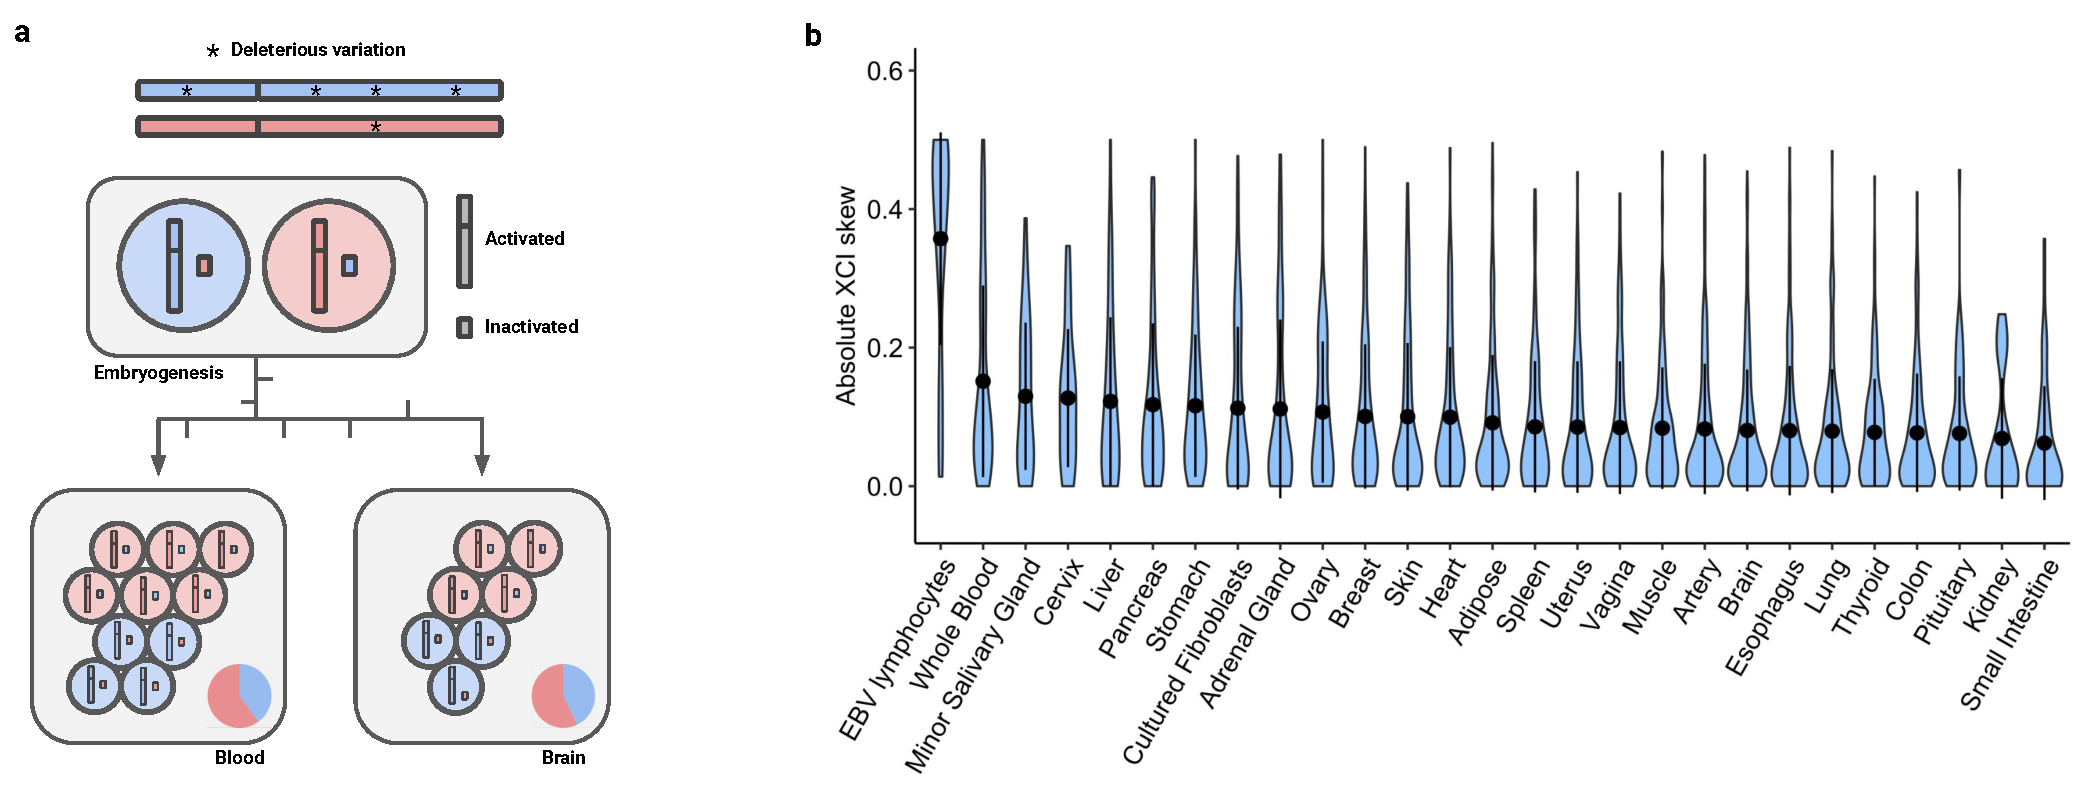
\includegraphics[width=\textwidth]{chapter4/Figures/Figure_1.pdf}
    \caption{
        Measuring XCI skew across tissues 
        \textbf{a}, Schematic overview of selection hypothesis. An individual inherits one haplotype (red) that is more fit than the other (blue) due to genetic variation. Given equal population sizes in embryonic development, we hypothesize that fitness differences will produce skewed populations in fully developed tissues.
        \textbf{b}, Violin plot of absolute XCI skew on the y-axis. Tissues are sorted by mean on the x-axis. Dots indicate mean of the absolute skew with vertical lines indicating one standard deviation.}
    \label{fig:fig4.1}
\end{figure}